\documentclass[tikz,border=0.0in]{standalone}
\usepackage{tikz}   
\usepackage{tikzscale}
\usepackage{amsmath}
\usepackage{graphicx}
\usetikzlibrary{arrows.meta, positioning}

\begin{document}

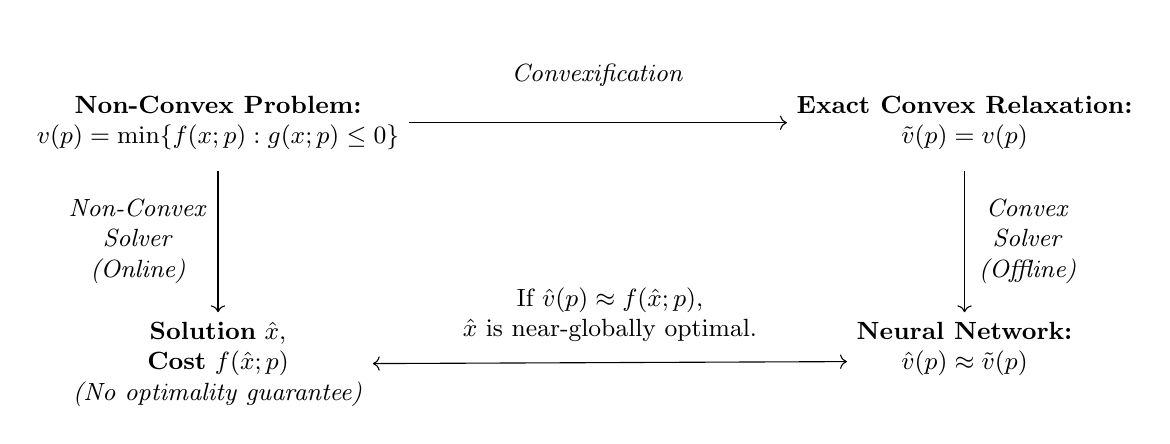
\begin{tikzpicture}[node distance=3.3cm and 4.8cm, every node/.style={rounded corners, minimum width=1.6cm, minimum height=1.2cm, align=center, font=\small}]
    \centering
    % Nodes
    \node (opf) {\textbf{Non-Convex Problem:}  \\ $v(p) = \min \{f(x;p) : g(x;p)\leq0\}$
    };
    \node[below =of opf, yshift=1.5cm] (local) {\textbf{Solution} $\hat{x}$, \\ \textbf{Cost} $f(\hat{x};p)$ \\ \textit{(No optimality guarantee)}};
    \node[right=of opf] (sdp) {\textbf{Exact Convex Relaxation:} \\ $\tilde{v}(p) = v(p)$};
    \node[below =of sdp, yshift=1.5cm] (global) {\textbf{Neural Network:} \\ $\hat{v}(p) \approx \tilde{v}(p)$ \\};

    % Arrows
    \draw[->] (opf) -- node[midway, left] {\textit{Non-Convex} \\ \textit{Solver} \\ \textit{(Online)}} (local);
    \draw[->] (opf) -- node[above] {\textit{Convexification}}(sdp);
    \draw[->] (sdp) -- node[midway, right] {\textit{Convex} \\ \textit{Solver} \\ \textit{(Offline)}} (global);
    \draw[<->] (global) -- node[above] {If $\hat{v}(p) \approx f(\hat{x};p)$, \\ $\hat{x}$ is near-globally optimal.} (local);
\end{tikzpicture}

\end{document}